
\chapter{Perspectives\label{chpt:perspectives}}

The work is never perfect, a great deal of unfinished work and theories
linked to this thesis is presented here. 

\section{Reduce memory footprint in MDFT}

The total CPU time to implement a \acs{MDFT} minimization using the
\texttt{\textbf{convolution}} algorithms is typically 1 to 30 minutes
according to the resolution of grid. But the memory consumed for such
a process is typically 1 to 20 G of RAM. This is mainly due to the
minimizer L-BFGS-B, which firstly needs to store several steps of
information during the iterations, and secondly is in double precision.
It is to say that the density variable $\rho(\mathbf{r},\mathbf{\Omega})$
and the gradient also need to be stored in double precision, and if
not, as I tested, it leads to divergence. In addition, during the
evaluation of the functional, the memory for at most 3 times $\rho(\mathbf{r},\mathbf{\Omega})$
needs to be open simultaneously.

There are two ways to get over this memory limit, and both of them
need to modify the L-BFGS-B minimizer, which is a ``blackbox'',
in Fortran 77. The simplest way is to change the double precision
to single in the L-BFGS-B minimizer; this action can reduce the memory
needed by a factor 2. Another way to completely pass this limit is
to parallelize the code to several nodes using MPI. This requires
only to modify the \acs{FFT} and L-BFGS-B process, where there is
a mixing of variables $\rho(\mathbf{r},\mathbf{\Omega})$. A third
route indeed would be to define a minimizer with much less memory
requirements.

\section{Site-based grid}

The \acs{IET} approach uses intermolecular spherical coordinates,
and cannot describe large molecules. As for \acs{MDFT} it uses a
homogeneous spatial grid, which has therefore the same resolution
near and far from the solute. The caveat of \acs{MDFT} is that the
3D grid needed should be relatively fine to produce satisfactory results
(typically 3-4 points per Angstrom); for large solutes this may lead
to a very huge number of grid points. A natural idea would be to use
non-uniform grids. One way to think about the construction of the
grid is like in \ref{fig:Site-site-grid-model}, a set of spherical
grids centered at each solute site. This could be understood as expanding
the density into a set of ``atomic-like orbitals'', $\rho(\mathbf{r})=\sum_{\alpha}c_{\alpha}\rho_{\alpha}(\mathbf{r})$.
Each ``'orbital'' could be possibly expanded onto a local basis
set, such as spherical harmonics, $\rho_{\alpha}(\mathbf{r})=\sum_{l,m}\rho_{\alpha,l}^{m}(|\mathbf{r}-\mathbf{R_{\alpha}}|)Y_{l}^{m}(\theta,\phi)$.

\begin{figure}[h]
\begin{centering}
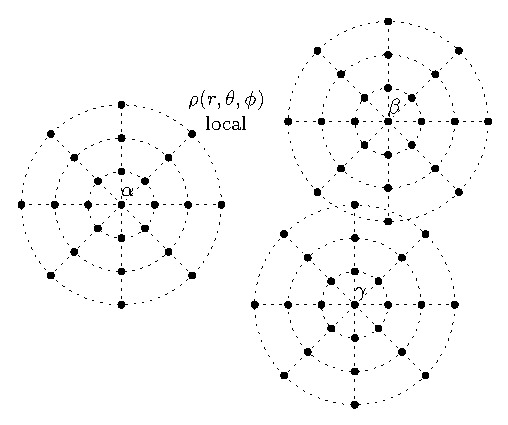
\includegraphics{_figure/site-site}
\par\end{centering}
\caption{Site-site grid model\label{fig:Site-site-grid-model}}
\end{figure}


\section{Theories beyond the HRF approximation and other improvements}

In terms of $\mathcal{F}_{\mathrm{exc}}$, there can still be development
beyond the \acs{HRF} approximation, such as 3-body corrections.

Apart from the $\mathcal{F}_{\mathrm{exc}}$ term, there are still
many fields of study to develop \acs{MDFT}. For example, the evaluation
of the external potential $V_{\mathrm{ext}}$ still poses occasional
problems of convergence for molecular solutes and needs to be improved.
Note also that the solute can be made polarizable, so that $V_{\mathrm{ext}}$
becomes itself a functional of the solvent density and varies during
the minimization. The polarization can be introduced, for example,
by an extra induced dipole on the solute center or on the solute sites.

\section{MDFT Viewer}

This thesis contained originally a contribution on visualization.
Due to time limit, it had to be removed. The Viewer is an important
part of the code development; it provides insightful visualization
and easier analysis, and may help to popularize the code. GaussViewer
is a good example.

\section{Application to real biological systems, and entropy}

From this thesis we can see that \acs{MDFT} is presently capable
to deal with small chemical system, but it is still far from satisfying
for common usage in the domain of bio-chemistry, or as a solvent model
for \acs{QM}. For example, for real applications, enthalpy and entropy
are also important, as discussed in ref \citep{Mn-oxo}. The properties
of \citep{Mn-oxo} cannot be repeated with \acs{QM} calculations
using simply a continuum model for solvent corrections (research subject
of my university diploma), which cannot reproduce the correct tendency
of entropy with respect to temperature (in DMSO). It is my intention
to re-investigate this problem using the \acs{MDFT} approach. It
is not clear yet how (beyond the estimate by the $\mathcal{F}_{\mathrm{id}}$
term), the solvation entropy rather than the free energy can be estimated
from the \acs{MDFT} calculations.
